\chapter{Methodology} \label{chap:methodology}
Position, orientation and velocities of a vehicle underwater are stored within the state vector. Proposed solution for localization uses state-space approach and Extended Kalman Filter (EKF, Chapter \S~\ref{chap:kalman}) to estimate the value of the state vector using data from odometric sensors and acoustic positioning system (LBL), if available. Data are merged together using the EKF. Reasons for choosing this method are influenced by the application itself. Localisation is intended to work in unstructured environments, with no clear visibility, relying on kinetic and absolute position measurements. Therefore, approaches that use vision, or capture the terrain structure in order to aid the navigation were not an adequate solution. Relying on the remaining sensor configuration allows the usage of Kalman filter to iteratively and recursively estimate the state vector by combining together different types of dynamics-related data. State-space approach is convenient for manipulation with multivariate data and nonlinear or non Gaussian processes \cite{ristic04}. Mathematical model of the system is the integral part of the Kalman filter. It is used to define the state transition law by applying well known kinematic equations.  Kinematic equations describe the object motion. \textit{Constant velocity} kinematic model is used as system model to predict the movements of the submerged body. States are predicted at each time-step using the model and previous state (equation ~\ref{eq:state-tran}). It is important to note that localization comes down to solving non-linear filtering problem. System model equations are nonlinear function of the state elements. Sensor measurements are used when available and incorporated into observation (measurement) in order to update and correct the predicted filter state. Range of available sensors give information on vehicle's current location state. Overview of the sensors and the values that they measure is given in Chapter \S~\ref{chap:sensors}.

\section{Process model} \label{sec:system-model}
5DOF system model is used to describe the state transition in time. In proposed discrete-time stochastic model, five degrees of freedom include position values and two angle states: yaw and pitch - making altogether five possible values to change in modelling vehicle position (figure ~\ref{fig:auv-positioning}). Since the application uses state-space approach, focus will be on defining a state vector that would incorporate all the relevant values for the dynamic system that does the localisation - kinematic and position variables. In spirit of that, system state vector combines together metric and angular values. At discrete time moment $k$, it values:
$$ \vect{X}(k) = 
\left[ 
\begin{array}{ccccccccccc}
x & y & z & a & u & v & w & \psi & \varphi & \dot{\psi} & \dot{\varphi}
\end{array}
\right] ^{T} $$  
where $x$ takes the value of \textit{north} (expressed in meters), $y$ is \textit{east} and $z$ is \textit{depth}. Inspiration for marking the variables with these letters was taken from \cite{ribas10}. Further on, $a$ marks the \textit{altitude} with $u$, $v$ and $w$ standing for linear velocities: \textit{surge velocity}, \textit{sway velocity} and \textit{heave velocity}, respectfully. The rest of the state vector covers angular values (expressed in radians or degrees). $\psi$ and $\varphi$ are used as yaw and pitch, hence describing the vehicle orientation. $\dot{\psi}$ and $\dot{\varphi}$ are angular velocities: yaw rate and pitch rate, respectfully. The state vector incorporates all the relevant information necessary to describe the system under investigation. Angle and velocity for pitch degree of freedom is included in 5DOF system model since it can make a difference in estimating vehicle location in certain movement scenarios (figure ~\ref{fig:motion-scenario}). System model is describing how the state $\vect{X}$ evolves in time. It is defined as constant speed model that uses previous state and noise to make a prediction on the next state vector value $\vect{X}(k)$  using non-linear function $f()$ and process noise vector $\vect{n}$ (equation ~\ref{eq:state-tran}) where $\vect{N} = \left[ \begin{array}{ccccc} \dot{u} & \dot{v} & \dot{w} & \ddot{\psi} & \ddot{\varphi} \end{array} \right]^{T}$. Process noise models inaccuracies or unpredictable disturbances in motion model \cite{ristic04}. 
\begin{equation}
\vect{X}(k) = f(\vect{X}(k-1), \vect{N}(k-1))
\label{eq:state-tran}
\end{equation}

\begin{equation}
\begin{bmatrix} x \\ y \\ z \\ a \\ u \\ v \\ w \\ \psi \\ \varphi \\ \dot{\psi} \\ \dot{\varphi} \end{bmatrix}_{(k)} =
\begin{bmatrix} x + (uT+\dot{u}\frac{T^{2}}{2})\cos(\psi)\cos(\varphi) - (vT+\dot{v}\frac{T^{2}}{2})\sin(\psi)\cos(\varphi) \\ 
                y + (uT+\dot{u}\frac{T^{2}}{2})\sin(\psi)\cos(\varphi) + (vT+\dot{v}\frac{T^{2}}{2})\cos(\psi)\cos(\varphi) \\ 
                z + (wT+\dot{w}\frac{T^{2}}{2})\cos(\varphi) \\ 
                a - (wT+\dot{w}\frac{T^{2}}{2})\cos(\varphi) \\ 
                u + \dot{u}T \\ 
                v + \dot{v}T \\ 
                w + \dot{w}T \\ 
                \psi    + \dot{\psi}T    + \ddot{\psi}   \frac{T^{2}}{2} \\ 
                \varphi + \dot{\varphi}T + \ddot{\varphi}\frac{T^{2}}{2} \\ 
                \dot{\psi}    + \ddot{\psi}T \\ 
                \dot{\varphi} + \ddot{\varphi}T
\end{bmatrix}_{(k-1)} 
\label{eq:state-tran-matrix}
\end{equation}
To summarize, implementing vehicle localization using EKF demands establishment of two models: first one describing the state evolution (system model) and second model that associates noisy measurement with the state (measurement model). 
\begin{figure}%[htb]
  \centering
    \subfigure[AUV positioning - global frame of reference.] {\label{fig:auv-positioning}
	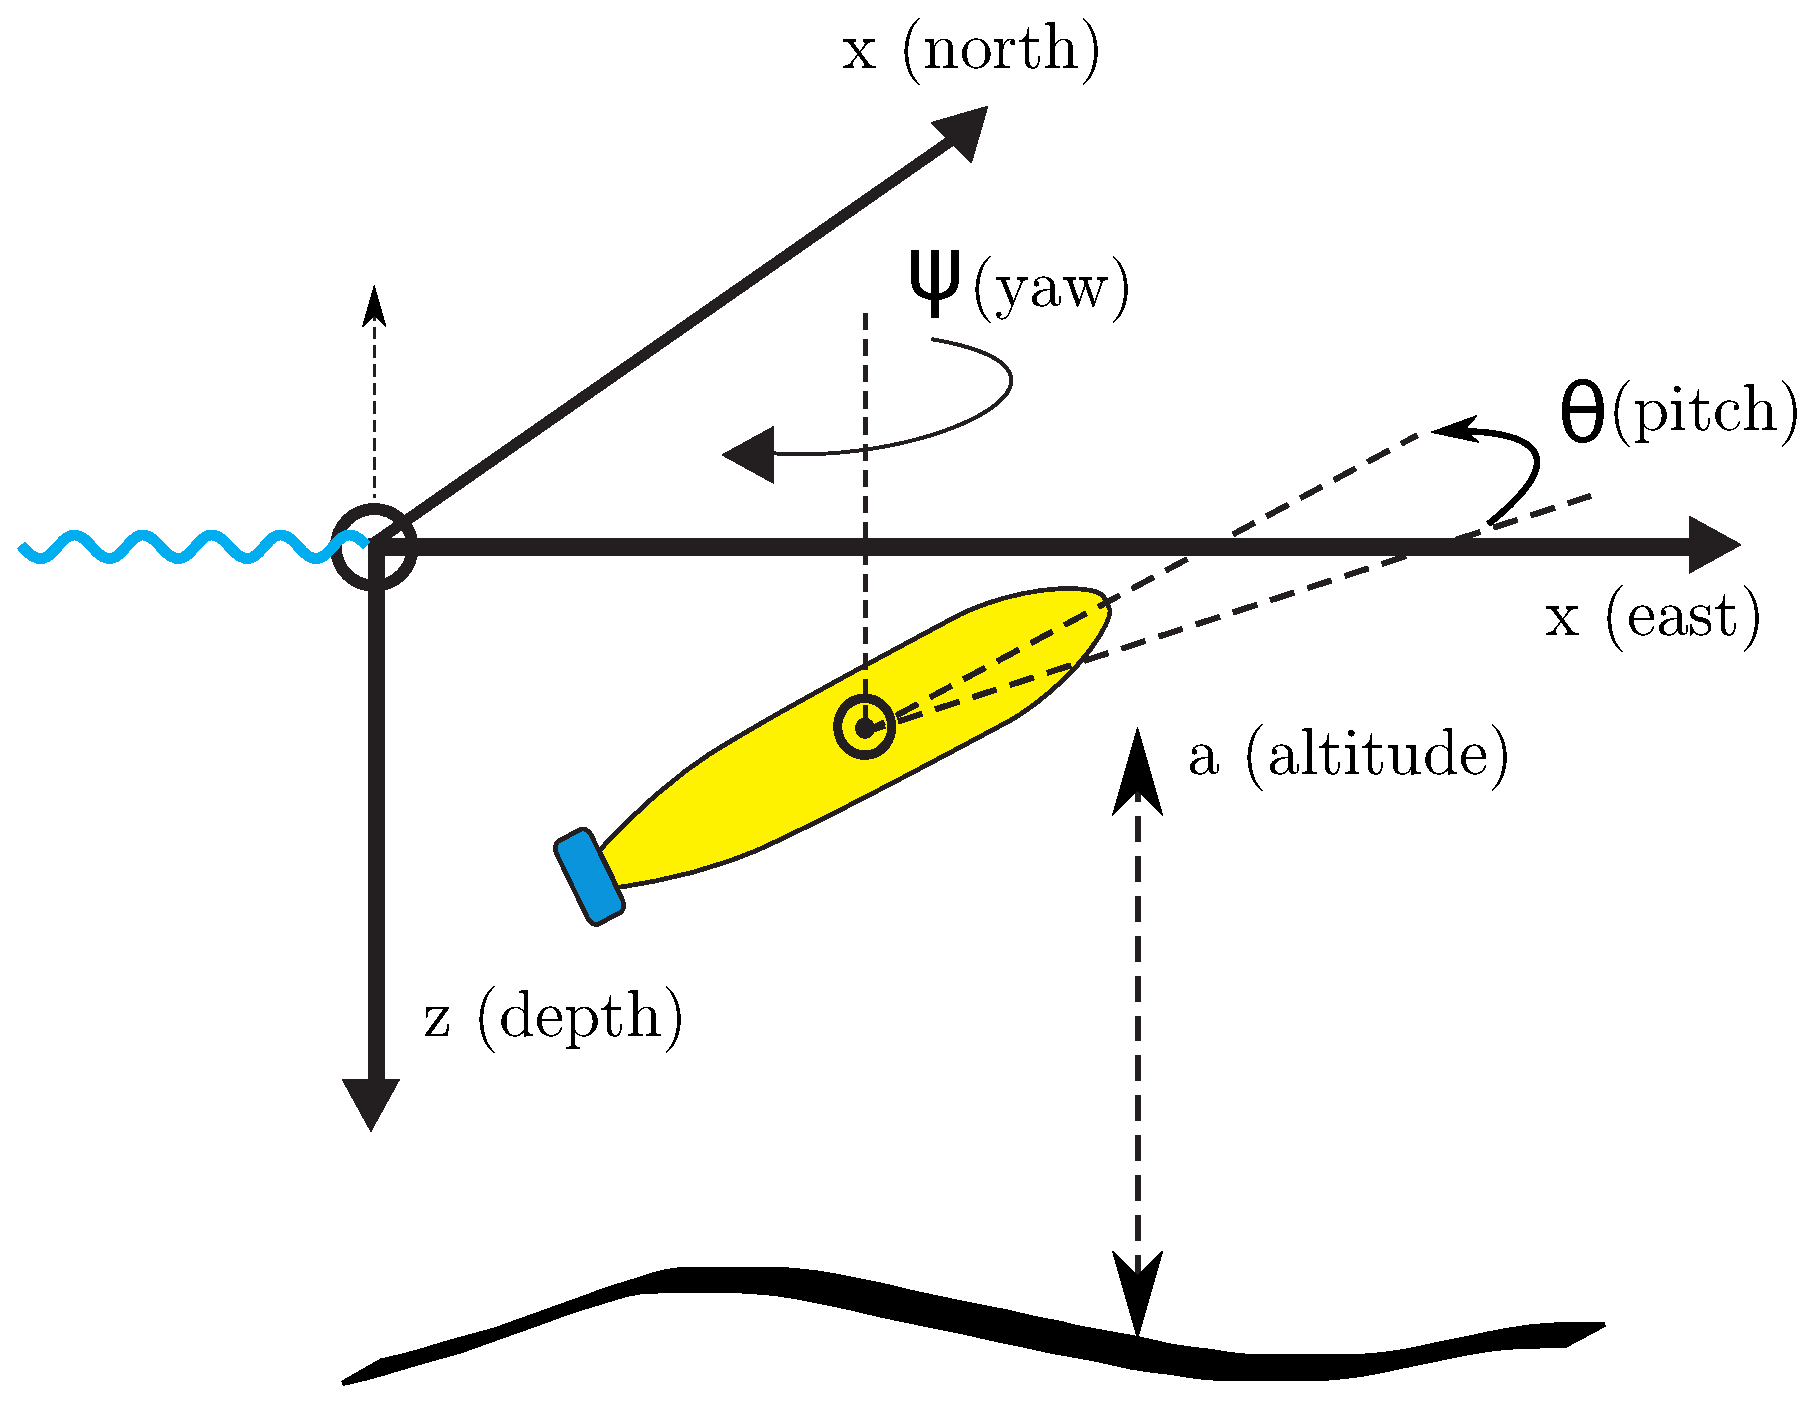
\includegraphics[width=0.40\linewidth]{methodology/fig/auv-model.eps}}
    \subfigure[AUV body frame - local coordinate system with movement directions.] {\label{fig:auv-axes}
    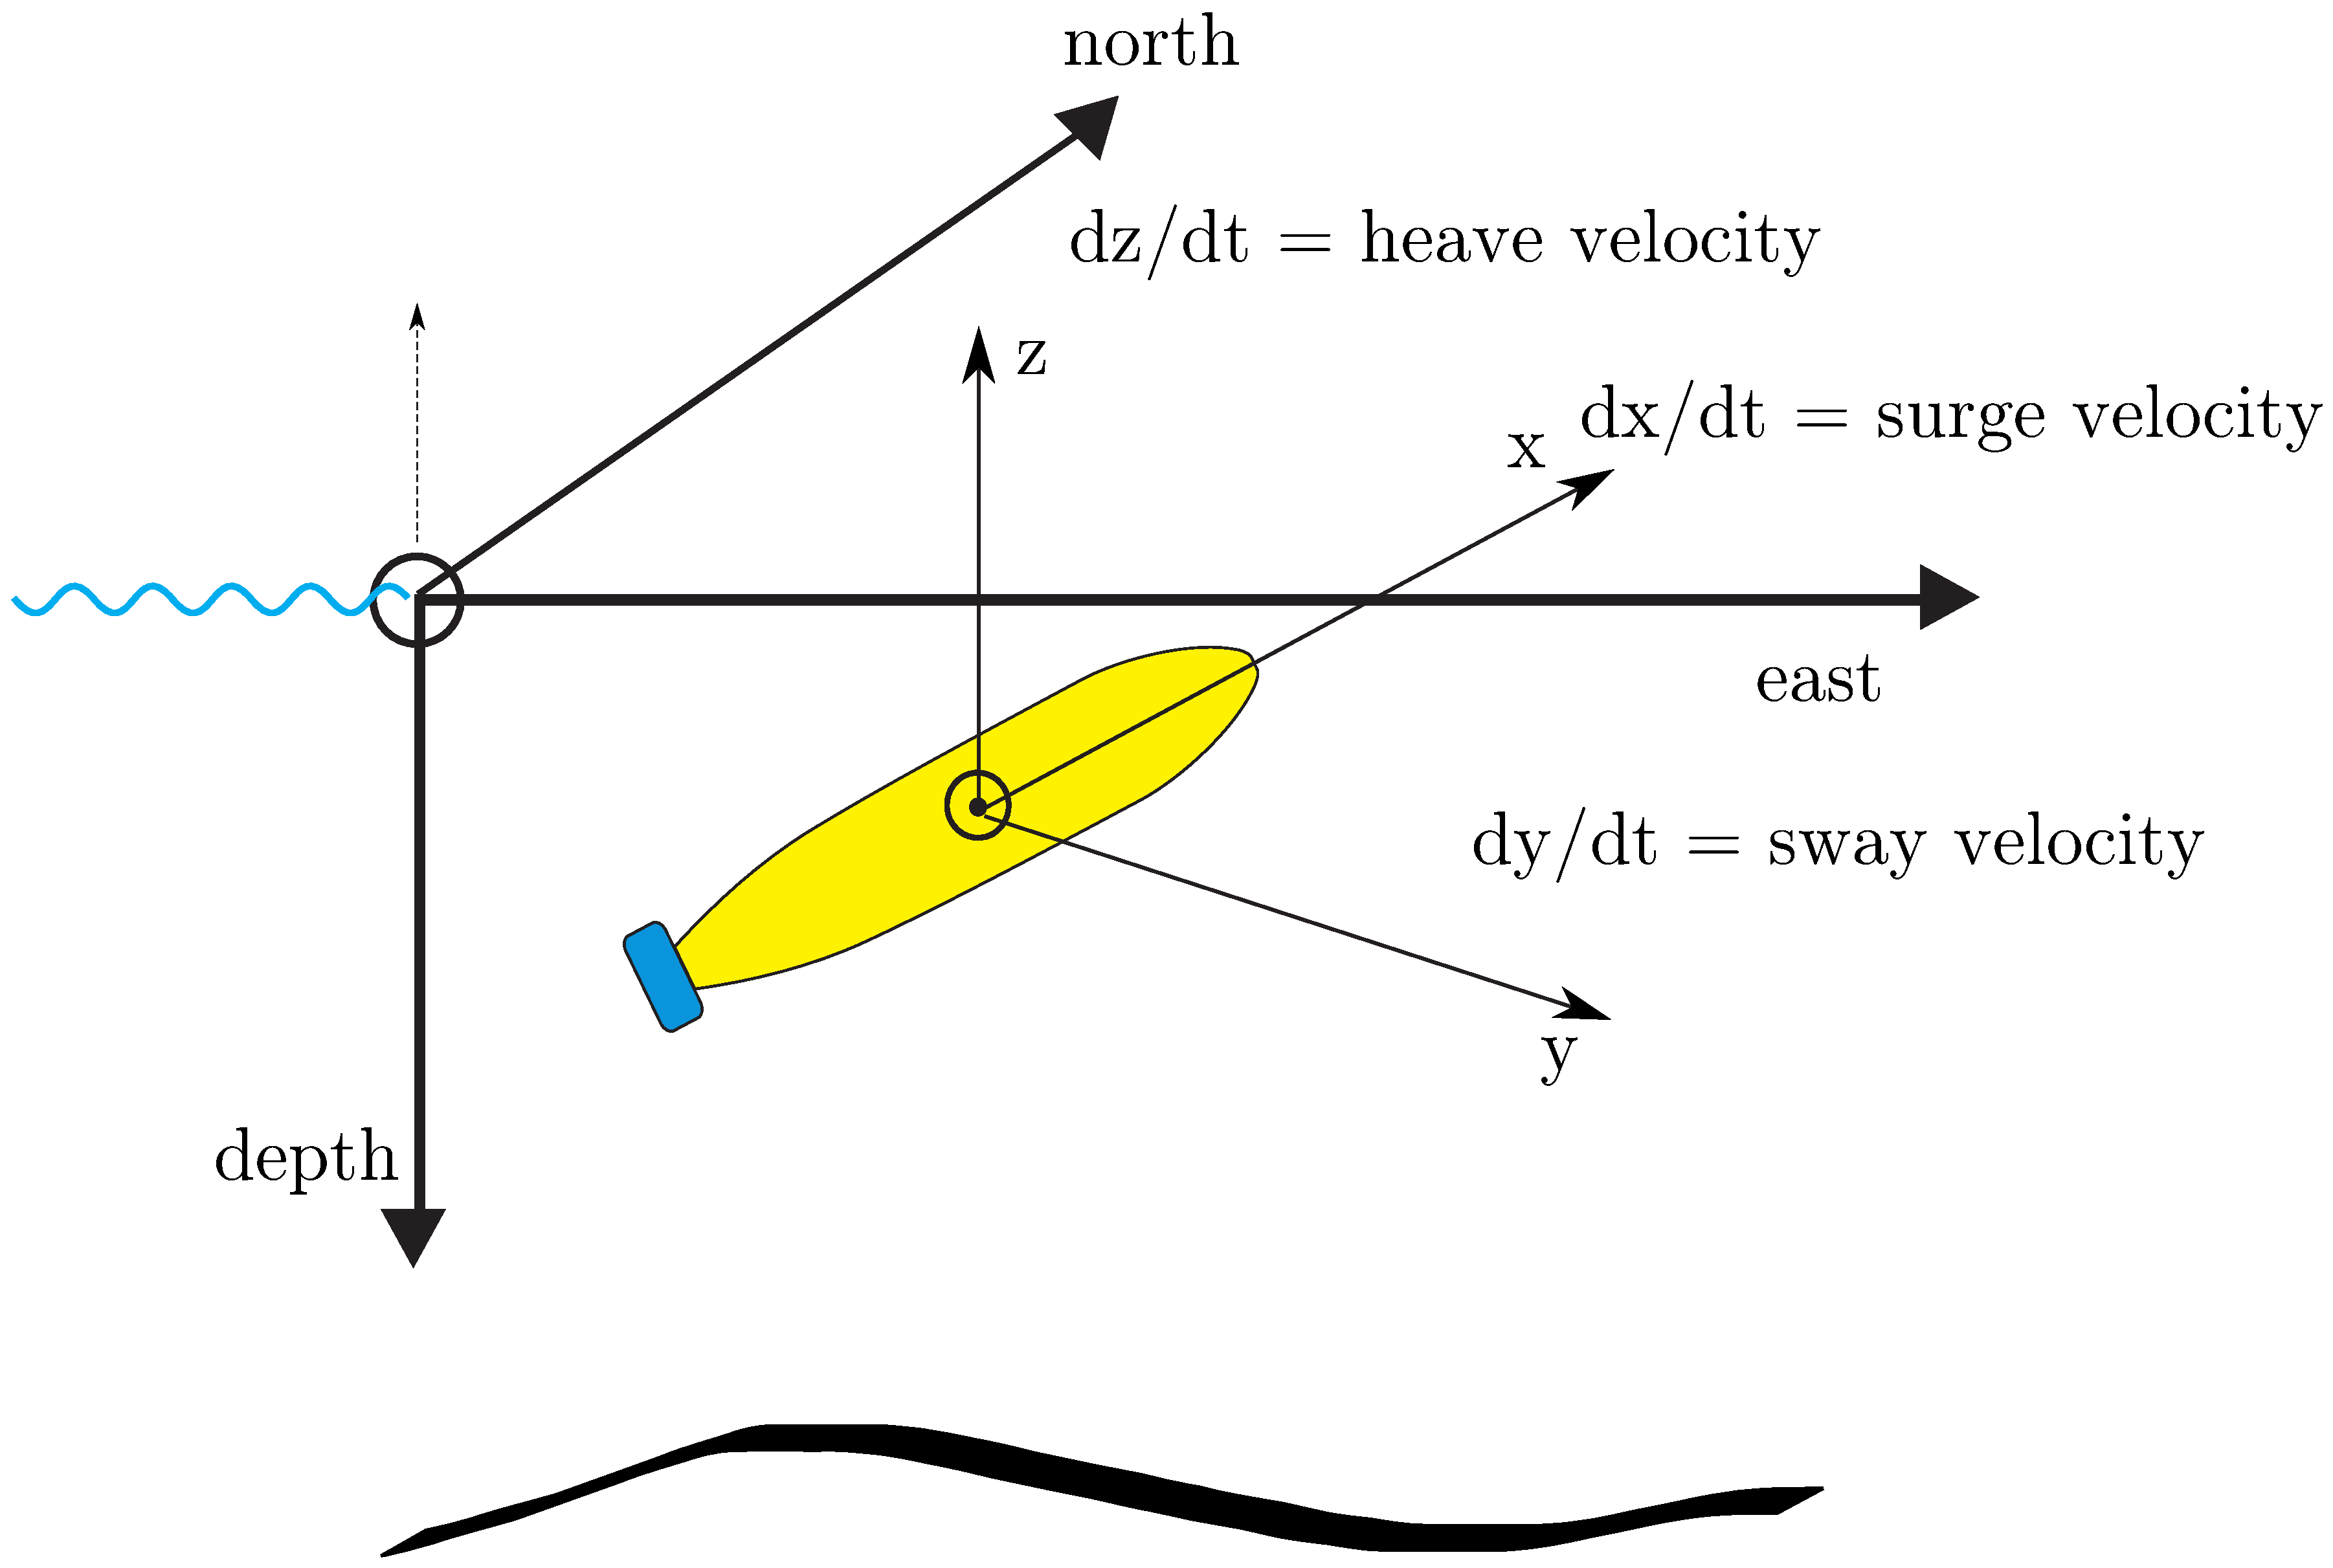
\includegraphics[width=0.40\linewidth]{methodology/fig/auv-axes.eps}} \\
    \subfigure[AUV pitch-influenced motion scenario.] {\label{fig:motion-scenario}
    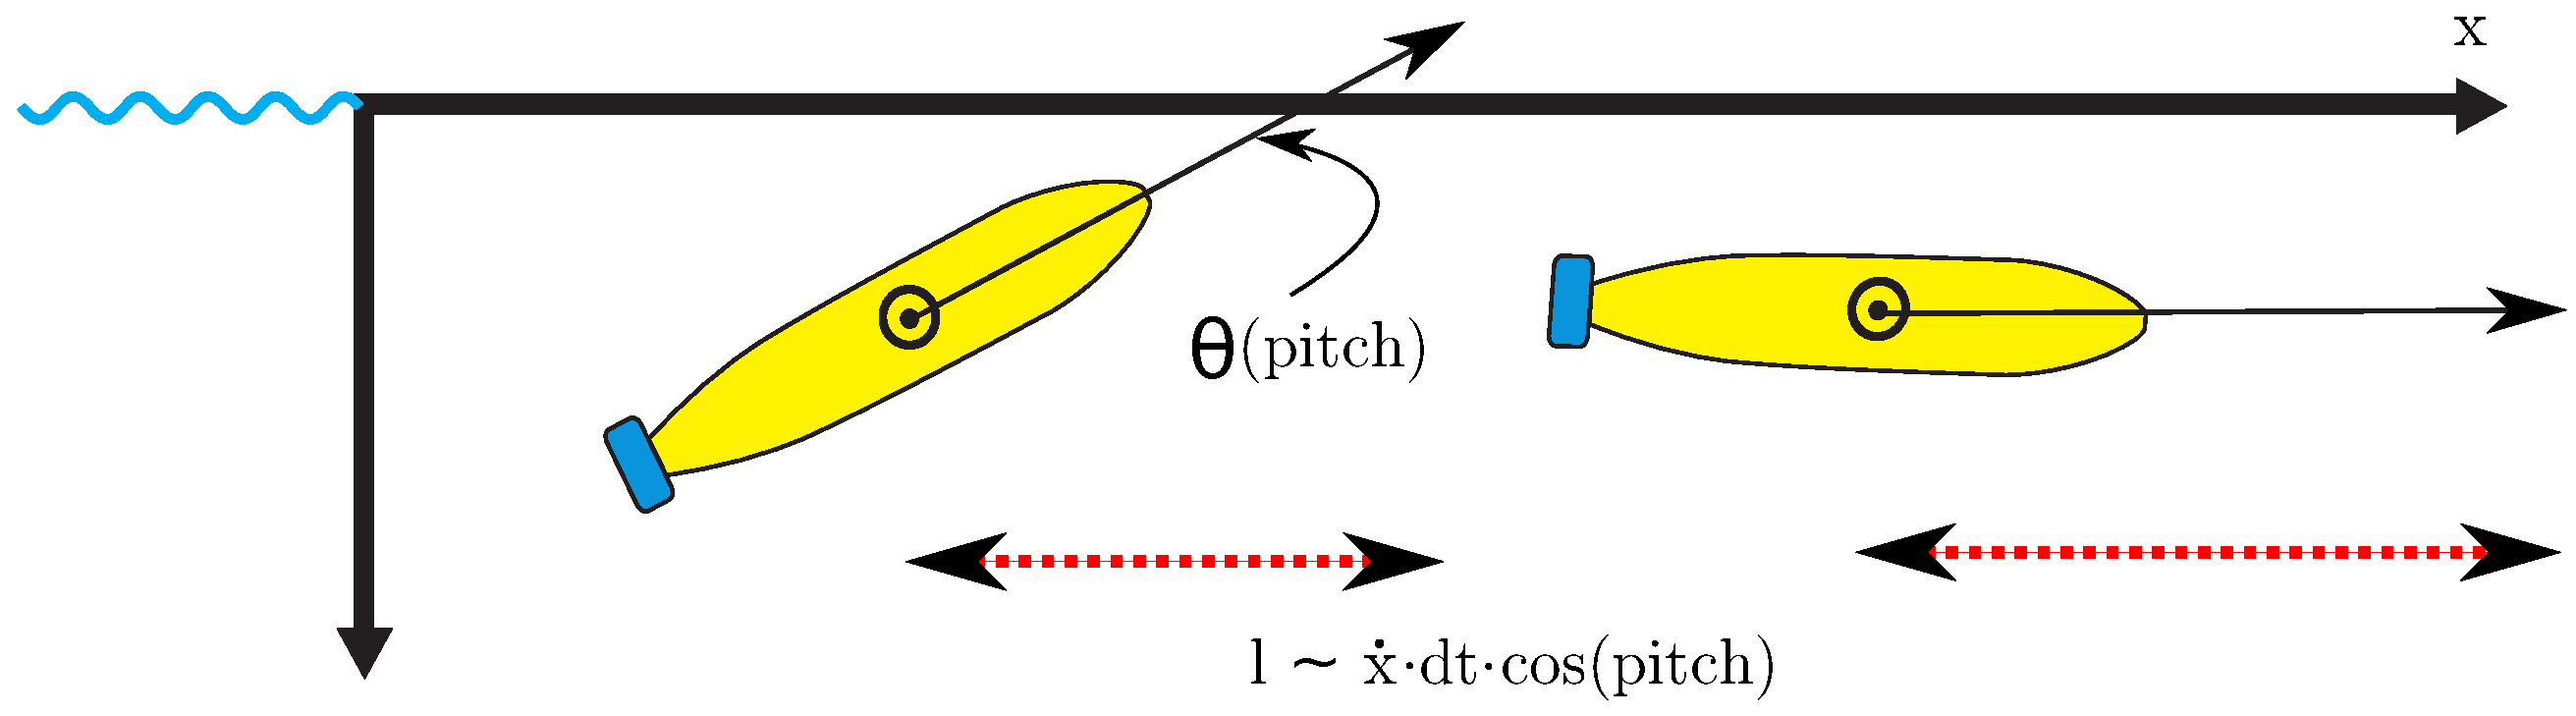
\includegraphics[width=0.5\linewidth]{methodology/fig/scenario.eps}}    
\caption{AUV state vector values and five degrees of freedom.}
\label{fig:auv-states}
\end{figure}

EKF (Chapter ~\ref{chap:kalman}) was used in order to estimate the vehicle state vector. It was chosen as logic choice being an algorithm that integrates together different sensor measurements, makes a sub-optimal, recursive state estimation and above all, is derived for non-linear systems. As the theory of non-linear filtering suggests, state-space approach is used for modelling discrete-time dynamic system in this application. The main feature of EKF is that it linearises the system model and measurement model nonlinear functions. System model is further developed according to formulas ~\ref{eq:der-proc-state}, ~\ref{eq:der-proc-noise}, ~\ref{eq:der-mes-state} and ~\ref{eq:der-mes-noise} from Chapter on Nonlinear filtering \S~\ref{chap:methodology}, resulting in matrices:
\begin{align*}
\vect{F}(k) & = &  \frac{\partial f}{\partial X} (\vect{\hat{X}}(k \mid k-1), 0) & = & 
\end{align*}
\begin{footnotesize}
$$ \left[ 
\begin{array}{ccccccccccc}
1 & 0 & 0 & 0 & T c(\psi) c(\varphi) & -T s(\psi) c(\varphi) & 0 & -Tc(\varphi)(us(\psi)+vc(\psi)) & -Ts(\varphi)(uc(\psi)-vs(\psi)) & 0 & 0 \\
0 & 1 & 0 & 0 & T s(\psi) c(\varphi) & T c(\psi) c(\varphi) & 0 & Tc(\varphi)(uc(\psi)-vs(\psi)) & -Ts(\varphi)(us(\psi)-vc(\psi))  & 0 & 0 \\
0 & 0 & 1 & 0 & 0 & 0 &  Tc(\varphi) & 0 & -vTs(\varphi) & 0 & 0 \\
0 & 0 & 0 & 1 & 0 & 0 & -Tc(\varphi) & 0 &  vTs(\varphi) & 0 & 0 \\
0 & 0 & 0 & 0 & 1 & 0 & 0 & 0 & 0 & 0 & 0 \\
0 & 0 & 0 & 0 & 0 & 1 & 0 & 0 & 0 & 0 & 0 \\
0 & 0 & 0 & 0 & 0 & 0 & 1 & 0 & 0 & 0 & 0 \\
0 & 0 & 0 & 0 & 0 & 0 & 0 & 1 & 0 & T & 0 \\
0 & 0 & 0 & 0 & 0 & 0 & 0 & 0 & 1 & 0 & T \\
0 & 0 & 0 & 0 & 0 & 0 & 0 & 0 & 0 & 1 & 0 \\
0 & 0 & 0 & 0 & 0 & 0 & 0 & 0 & 0 & 0 & 1 \\
\end{array}
\right] $$ 
\end{footnotesize}
where $c(\psi)$ and $c(\varphi)$ stand for $\cos(\psi)$ and $\cos(\varphi)$ respectfully. Similarly, $s(\psi)$ and $s(\varphi)$ mark the angle sinuses.  
\begin{align*}
\vect{W}(k) & = \frac{\partial f}{\partial N} (\vect{\hat{X}}(k \mid k-1), 0) & = &
\end{align*}
$$ 
\begin{bmatrix}
\frac{T^{2}}{2}\cos(\psi)\cos(\varphi) & -\frac{T^{2}}{2}\sin(\psi)\cos(\varphi) & 0 & 0 & 0 \\
\frac{T^{2}}{2}\sin(\psi)\cos(\varphi) &  \frac{T^{2}}{2}\cos(\psi)\cos(\varphi) & 0 & 0 & 0 \\
0 & 0 & \frac{T^{2}}{2}\cos(\varphi) & 0 & 0 \\
0 & 0 & -\frac{T^{2}}{2}\cos(\varphi) & 0 & 0 \\
T & 0 & 0 & 0 & 0 \\
0 & T & 0 & 0 & 0 \\
0 & 0 & T & 0 & 0 \\
0 & 0 & 0 & \frac{T^{2}}{2} & 0 \\
0 & 0 & 0 & 0 & \frac{T^{2}}{2} \\
0 & 0 & 0 & T & 0 \\
0 & 0 & 0 & 0 & T \\
\end{bmatrix}
$$
Knowing plant model and deriving $\vect{F}(k)$, $\vect{W}(k)$ enables EKF algorithm to complete the prediction stage using known formulas. Next step is correction of the prediction using data obtained from measurement.
\section{Measurement model} \label{sec:measurement-model}
Measurement model introduces measurement equation which establishes connection between the measurements and the target state (equation ~\ref{eq:mes-model}) where $Z(k)$ represents the measurement at time $k$, $X(k)$ represents state vector and $M(k)$ represents noise. Purpose of the measurement is to be able to update, correct the state $X(k)$ using measurements $Z(k)$. $h()$ is generally a non-linear function. EKF idea is to linearise measurement model.
\begin{align*}
\vect{H}(k) = \frac{\partial h}{\partial X} (\vect{\hat{X}}(k \mid k-1), 0) \\
\vect{R}(k) = \frac{\partial h}{\partial M} (\vect{\hat{X}}(k \mid k-1), 0)
\end{align*}
However, for this particular application and available sensor configuration, state vector elements are measured directly, hence $h()$ can be expressed with matrix containing ones at particular positions since the measurement relation becomes equality. There is no need for partial derivation. Measurement noise is submitted in form of additive Gaussian zero-mean noise assigned to each measured value. Measurement (observation) noise is characterised with zero mean $(E \lbrace \vect{M}(k) \rbrace = 0)$ and standard deviation $(E \lbrace \vect{M}(k) \vect{M}^{T}(k) \rbrace)$ given as filter parameter for each of the measurement. It expresses how uncertain or varying, measurement of each of the state values is. The measurement in vehicle configuration used for the thesis enables direct measurement of each of the states and each measurement of one of the state elements is described with its uncertainty - variance of the Gaussian noise. Variances are given as filter parameters saying how much we trust in the measurement.  
\begin{equation}
\vect{Z}(k) = h(\vect{X}(k), M(k)) = \vect{H} \vect{X}(k \mid k-1)  + \vect{M}(k)
\label{eq:mes-model}
\end{equation}
One of the features of EKF localization for an AUV is that measurements are not available all the time. Reason is the nature of the process of estimating localization itself. Simply - messages from sensors arrive at different moments and it happens that some of the sensors could not be available due to different causes. The idea is to take all the available information at the moment of filtering and integrate it together in measurement model, as filter observation. Alternatively, each message can be filtered upon its arrival. As a result, filter would keep carrying out the prediction and correction blending together various measurements in a estimate of higher quality, with the ability to compensate the missing sensor measurements. 

A short overview of the sensor measurements and the pattern of formation of the measurement model is presented in following section. Idea for the solution has been introduced in \cite{ribas10}. Some other implementations of EKF for underwater navigation have reported the usage of similar strategy for merging the measurements together \cite{drolet00, blain03}. Sensors have been introduced with more details in chapter ~\ref{chap:sensors}. Linear observation model varies depending on the measured values and sensors used for the measurement. 
\begin{itemize}
\item \T{Pressure sensor}
periodically ``feeds'' the filter with depth and heave velocity information. Heave velocity information is derived from depth measurement by derivation of its value per elapsed time. Measurement model is linear, described with the transformation matrix $\vect{H}_{depth}$. Uncertainty of the measurement is expressed with measurement noise matrix $\vect{R}$ (EKF, chapter ~\ref{chap:kalman}) - covariance of the measurement vector.  
\begin{equation}
\label{eq:press-mes}
\vect{H}_{depth}(k) = 
\left[ \begin{array}{ccccccccccc}
0 & 0 & 1 & 0 & 0 & 0 & 0 & 0 & 0 & 0 & 0 \\
0 & 0 & 0 & 0 & 0 & 0 & 1 & 0 & 0 & 0 & 0 \end{array} \right],
\vect{R}_{depth}(k) =  
\left[ \begin{array}{cc}
\sigma_{z}^{2} & 0 \\
0 & \sigma_{w}^{2} \end{array} \right]
\end{equation}
\item \T{Compass}
supplies angular measurements such as pitch, yaw, pitch rate (figure ~\ref{fig:auv-positioning}). Similarly as with pressure sensor measurement model, rate of change of pitch is obtained with derivation of pitch measurement. Measurement model is linear, described with the transformation matrix $\vect{H}_{compass}$. $\vect{R}_{compass}$ is measurement noise matrix (EKF, chapter ~\ref{chap:kalman}) containing variances depicting Gaussian noise of particular measurements.
\begin{equation}
\label{eq:com-mes}
\vect{H}_{compass}(k) = 
\left[ \begin{array}{ccccccccccc}
0 & 0 & 0 & 0 & 0 & 0 & 0 & 0 & 1 & 0 & 0 \\
0 & 0 & 0 & 0 & 0 & 0 & 0 & 0 & 0 & 0 & 1 \\
0 & 0 & 0 & 0 & 0 & 0 & 0 & 1 & 0 & 0 & 0 \end{array} \right], 
\vect{R}_{compass}(k) =
\left[ \begin{array}{ccc}
\sigma_{\varphi}^{2} & 0 & 0 \\
0 & \sigma_{\dot{\varphi}}^{2} & 0 \\
0 &     0          & \sigma_{\psi}^{2} \end{array} \right]
\end{equation}
\item \T{Fiber-optic-gyroscope sensor (FOG)}
measures yaw rate $(\dot{\psi})$. FOG, unlike compass, gives an absolute measurement of the rate. In case of compass yaw rate is determined by doing derivation in time using previous yaw measurement. FOG turns out to be quite precise and fast sensor. Yaw rate can be used to determine the yaw (heading) itself by integrating the yaw rates over time. That would imply relative measurement of yaw - with respect to previous value. Relative measurements cannot correct the starting error, in case it existed.  Disadvantage of FOG usage for yaw measurement is that the initial heading value still needs to be given by compass, as an absolute measurement. This can result in constant bias of measured heading in case the initial heading was measured with an error. Error would propagate through relative measurements in form of the bias. Given that compass is prone to errors, this scenario is possible. Measurement model matrices are:
\begin{equation}
\label{eq:fog-mes}
\vect{H}_{fog}(k) = 
\left[ \begin{array}{ccccccccccc}
0 & 0 & 0 & 0 & 0 & 0 & 0 & 0 & 0 & 1 & 0  \end{array} \right], 
\vect{R}_{fog}(k) =
\left[ \begin{array}{c}
\sigma_{\dot{\psi}}^{2} \end{array} \right]
\end{equation}  
\item \T{Doppler Velocity Log (DVL)}
measures linear speeds - surge and sway velocities with respect to vehicle axes (Figure ~\ref{fig:auv-axes}) and the altitude. $\vect{H}_{dvl}$ and $\vect{R}_{dvl}$ are measurement and measurement noise matrices (EKF, chapter ~\ref{chap:kalman}) containing variances depicting Gaussian noise of particular measurements. If DVL gives no valid velocity output due to insufficient signal (DVL lock lost), EKF is using the available data available from other sensors to make an update or it is just maintaining the increasingly uncertain prediction part until the fresh observation arrives.    
\begin{equation}
\label{eq:dvl-mes}
\vect{H}_{dvl}(k) = 
\left[ \begin{array}{ccccccccccc}
0 & 0 & 0 & 1 & 0 & 0 & 0 & 0 & 0 & 0 & 0 \\
0 & 0 & 0 & 0 & 1 & 0 & 0 & 0 & 0 & 0 & 0 \\
0 & 0 & 0 & 0 & 0 & 1 & 0 & 0 & 0 & 0 & 0 \end{array} \right], 
\vect{R}_{dvl}(k) =
\left[ \begin{array}{ccc}
\sigma_{a}^{2} & 0 & 0 \\
0 & \sigma_{u}^{2} & 0 \\
0 &     0          & \sigma_{v}^{2} \end{array} \right]
\end{equation}
\item \T{Long-baseline (LBL)}
gives an absolute position update based on GPS signal from surface as reference and triangulation obtained from transponders with known global position place around the vehicle (figure ~\ref{fig:standard-lbl}). This serves as a crucial anti drift tool because it is not relative to previous measurements. It results in fresh update of global position in form of latitude and longitude that can be mapped into north and east of the local position in meters. Algorithmically, this can be regarded as an update of north and east causing matrices of measurement update to become:
\begin{equation}
\label{eq:lbl-mes}
\vect{H}_{lbl}(k) = 
\left[ \begin{array}{ccccccccccc}
1 & 0 & 0 & 0 & 0 & 0 & 0 & 0 & 0 & 0 & 0 \\
0 & 1 & 0 & 0 & 1 & 0 & 0 & 0 & 0 & 0 & 0 \end{array} \right], 
\vect{R}_{lbl}(k) =
\left[ \begin{array}{cc}
\sigma_{n}^{2} & 0  \\
0 & \sigma_{e}^{2}  \end{array} \right]
\end{equation}
\item \T{GPS}
similarly as LBL, directly outputs a fairly accurate position measurement. GPS signal is not available underwater, hence, it is used at the beginning of the mission, when the vehicle is still on the surface, to establish the initial estimate. Algorithm keeps the track of all the GPS messages received, and in case the vehicle reaches the surface after deployment being able to receive GPS signal - that information is used to update the absolute position and correct the dead reckoning drift that happened meanwhile. Kalman fiter matrices keep the same form as with the LBL, uncertainties can be set to different values.
\end{itemize}

Once having the measurement, it is important to know its strategy of integration. Kalman filtering is intended to work in two modes:
\begin{itemize}
\item \T{asynchronous}
filtering messages from each sensor individually upon retrieval. Observation uses only measurements form each sensor individually. Every time sensor device produces a new output, all the localization variables are updated.
\begin{figure}%[htp]
  \begin{center}
    \subfigure[EKF filters after each sensor measurement.]   {\label{fig:asynch}   
    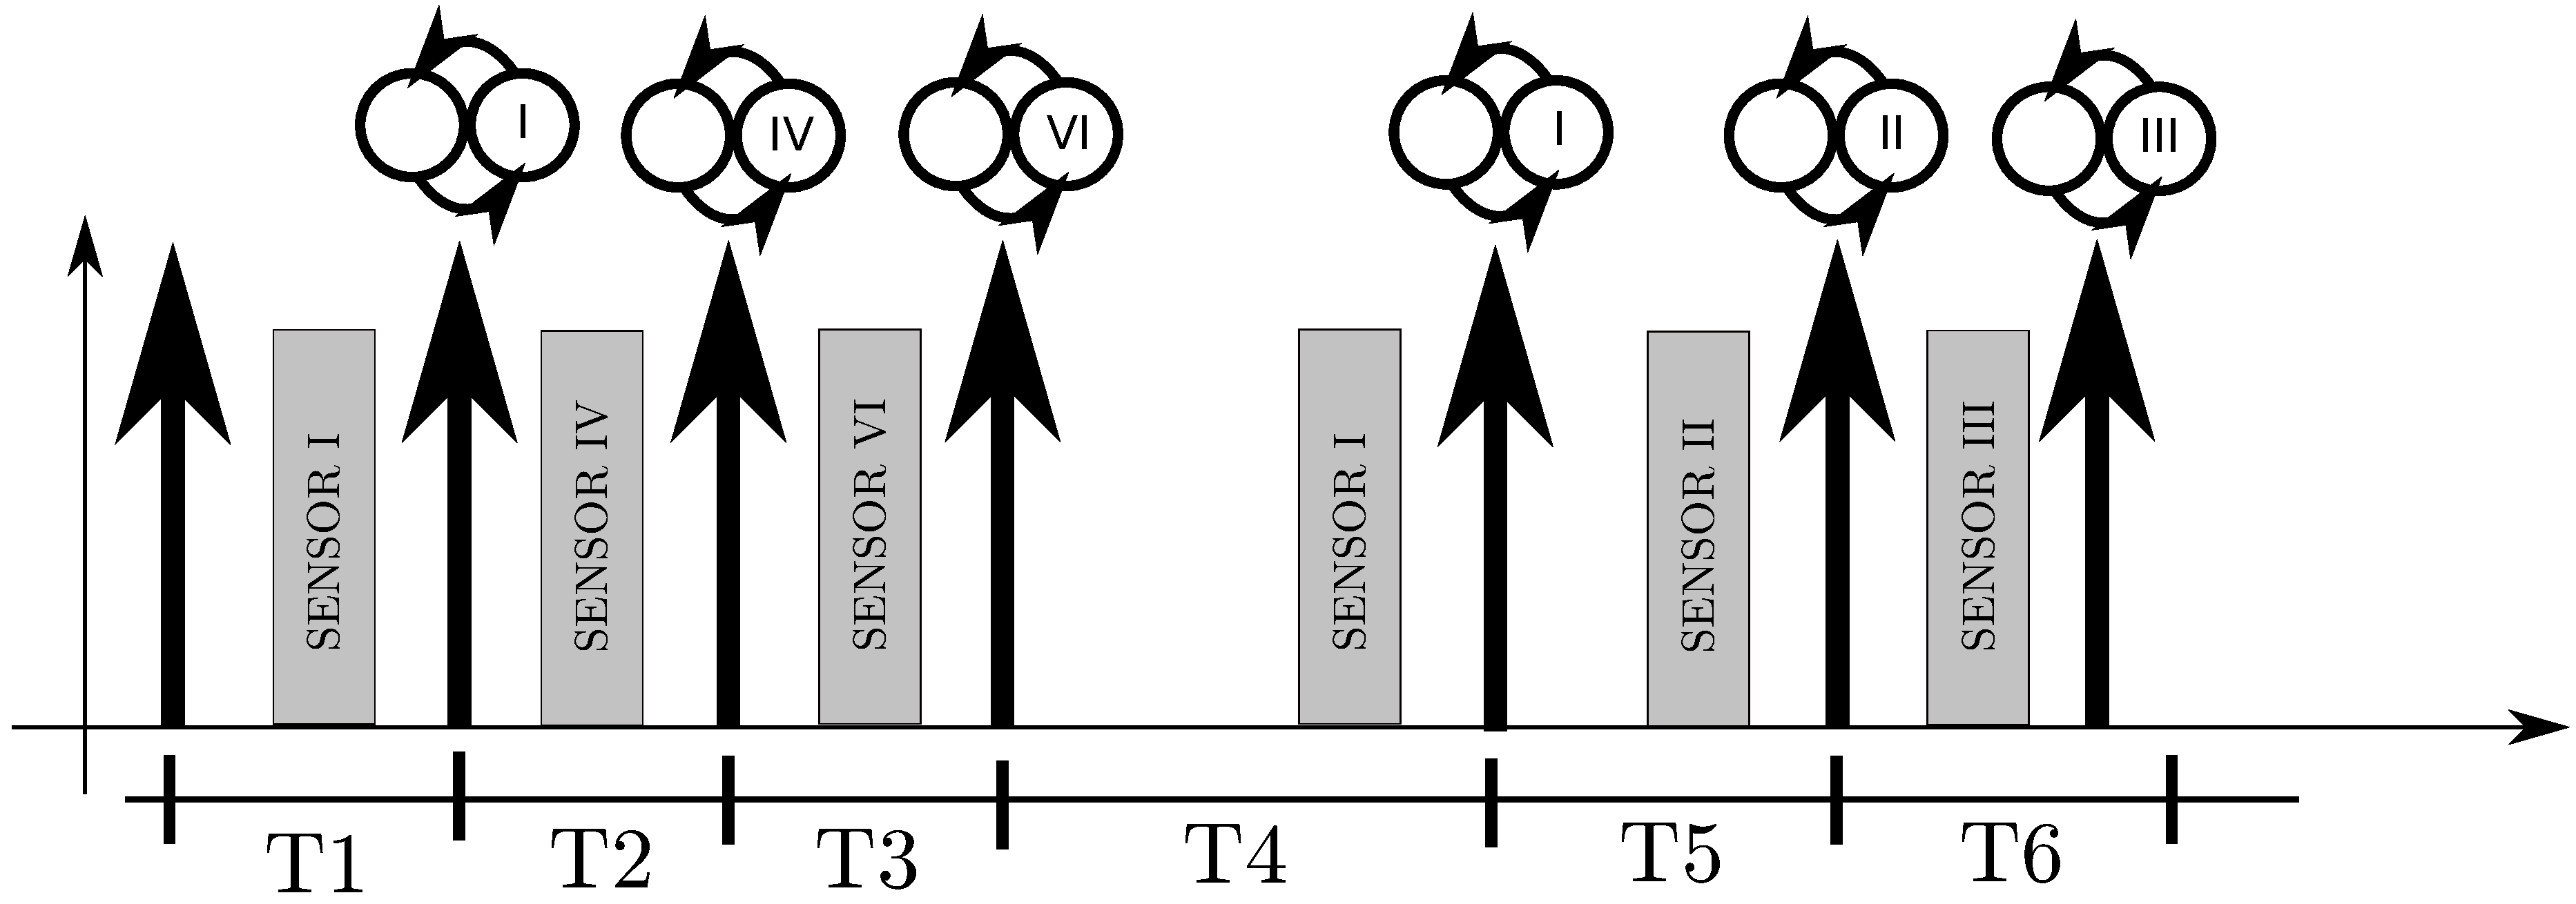
\includegraphics[width=0.7\textwidth]{methodology/fig/asynch.eps}}
    \subfigure[EKF filters periodically.]{\label{fig:synch}
    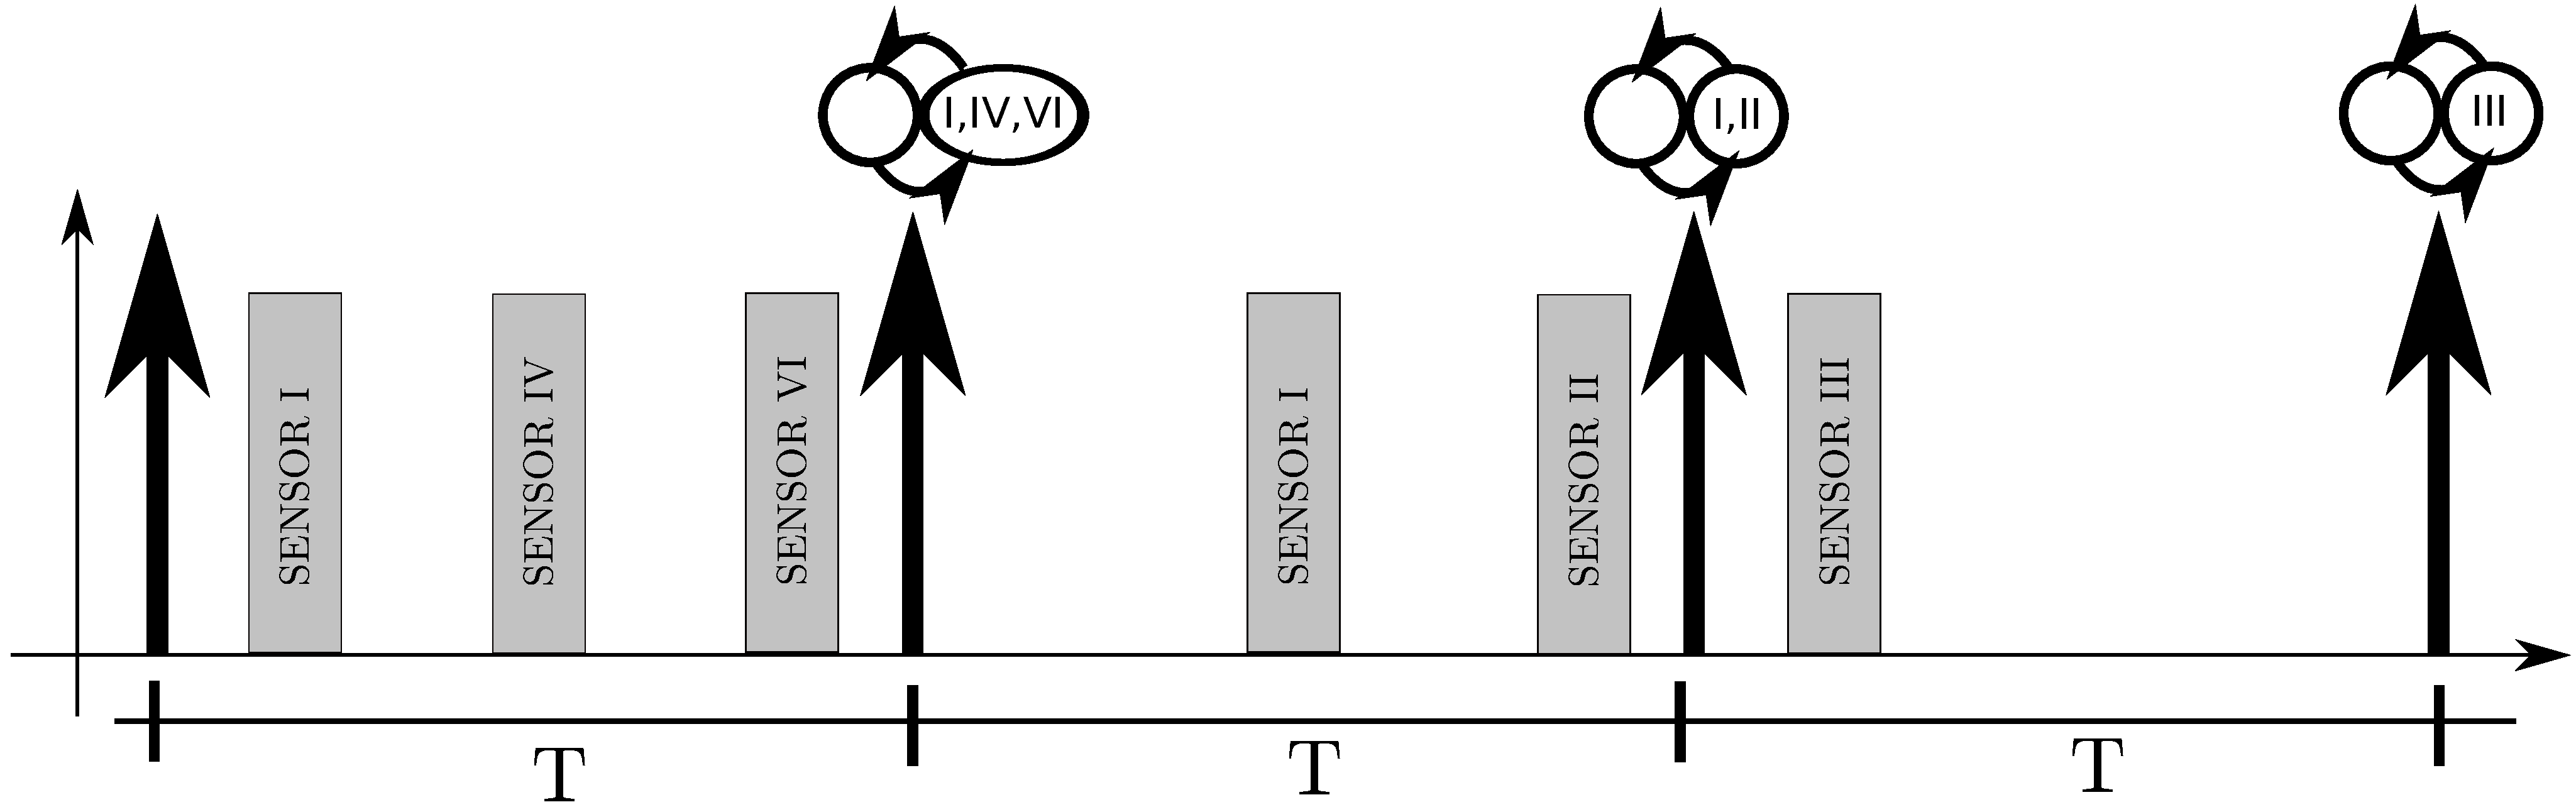
\includegraphics[width=0.7\textwidth]{methodology/fig/synch.eps}}  
  \end{center}
  \caption{Two modes for combining together sensor measurements into observation.}
  \vspace{-10pt}
  \label{fig:ekf-modes}
\end{figure}
\item \T{synchronous}
periodically updating with the most recent observation that combines together measurements from different sensors that occurred since the last update. User defined rate will determine the interval of the update.
\end{itemize}
Integrating together several different measurements into one observation would imply combining together several measurement $(\vect{Z}, \vect{H})$ and measurement noise matrices $(\vect{R})$, as shown in ~\ref{eq:concatenate-mes} for the sample case of three sensor measurements included in observation. Kalman filter maintains its own timer. Observation is reset after each timer set period.  
\begin{equation}
\label{eq:concatenate-mes} 
\vect{Z}(k) = \left[ \begin{array}{c} \vect{Z}_{sensor I} \\ \vect{Z}_{sensor II} \\ \vect{Z}_{sensor III} \end{array} \right],
\vect{H}(k) = \left[ \begin{array}{c} \vect{H}_{sensor I} \\ \vect{H}_{sensor II} \\ \vect{H}_{sensor III} \end{array} \right], 
\vect{R}(k) = \left[ \begin{array}{ccc} \vect{R}_{sensor I} & 0 & 0 \\ 0 & \vect{R}_{sensor II} & 0 \\ 0 & 0 & \vect{R}_{sensor III} \end{array} \right]
\end{equation}
Literature offers different approaches in managing Kalman filter update and managing observations. Matrix concatenation is used to gather together all the measurements into one observation. In case certain sensor measurement repeats during the update interval, the most recent measurement takes place of its preceding one within the periodic observation. This substitution is fairly realistic to happen, knowing that the user chooses filter update interval and that sensor devices have a range of frequencies, possibly more frequent that filter itself (table ~\ref{tab:sensors-char}). Simply put, observation is a buffer that stores the most recent collection of different measurements that occurred in meanwhile. Depending on the mode of operation (asynchoronous or synchrononus) the observation can contain the measurement from an individual sensor or those sensors that were active during the predefined period $T$ of update (Figure ~\ref{fig:synch}). Choosing the newest measurement is advantage from the point of having the most recent value as measurement, especially if the Kalman update interval is longer. However, it can also be a disadvantage in situations when certain sensor measurements happen at the beginning of the observation interval. For those ``earlier'' measured values, prediction stage will use less accurate time-stamp in EKF and the measurement itself would suit reality less, since it's usage is delayed. This effect is visible if update periods of EKF are long, which is not common case.  

Having more than one measurement involved in estimation of the global state is a good characteristic. The estimate which uses more diverse data gives better estimate since it is possible to combine together more that one sort of observation. Another advantage follows the fact that the whole set of state variables is updated each time, resulting in more correlation between variables. Hence those that are missing for some reason can be compensated this way. Results of simulations using authentic data and the  real misssions are given in Chapter \S~\ref{chap:results}. 
%\section{Non-linear Kalman Filter}
%By implementation standard filtering techniques such as the non-linear Kalman filtering or ``unscented'' filtering, one can obtain a minimum mean squared error estimate of the state conditioned upon all observations up to current time.
\section{Correction}
IMU is integrating acceleration or speed data collected from devices such as gyroscope or accelerometers. Integration of noisy data over time time or usage of ``relative measurements'' (those calculated from absolute measurements) results in drift or bias of the final estimate. In order to recover from that, algorithms perform correction. Correction takes an absolute measurement which should be less precise, possibly noisy, but not prone to drifting. An example which illustrates the phenomenon could be a man that walks with the eyes closed and tries to keep the track of his position by measuring the steps and predicting where he could possibly be judging on number of steps and their size. Steps have the role of ``relative measurement'' - one quantity is used to estimate the other one that's correlated with it. Naturally, a man will keep making errors in his position estimate. Moreover, these errors will accumulate over time producing drift. Correction would require man to open his eyes and observe the current position (absolute measurement), compare it with the position predicted by counting steps and neutralise the drift before carrying on with the eyes closed. 
\section{Sensor fusion}
Localization algorithm collects the incoming sensor information and computes the pose of the vehicle by processing the whole data cluster obtained from sensor devices. Such procedure is regarded as \textit{sensor fusion}. Basic sort of sensor fusion implementation is incorporated in navigation algorithm by combining different quantities into a jointly updated state vector.
\section{Implementation} \label{sec:implementation}
Localisation algorithm was planned to be part of navigation module of Ocean System Lab's Nessie vehicle. Vehicle's real-time operating system is Linux (Unix). Designing navigation requires programming the module using C++ programming language, conforming with available libraries. The aim is to produce an applicable module that fits in the existing software system and accomplishes the task theoretically explained in this chapter. In addition, Nessie is supported with Robot Operating System (ROS, \url{http://www.ros.org/wiki/}) - meta operating system that manages various processes maintained on vehicle and the real-time exchange of data between different modules. Hence, EKF navigation is implemented as a ROS package tailored to Nessie's messaging and processing scheme. 

One of the issues that need to be corrected when working with angles is angle wrapping. It is an inevitable issue in Kalman Filter implementations that involve angular values stored in the state vector. Fact is that filtering does calculations with angular values. Moreover, angular functions are $2\pi$ periodical. Because they are periodical, it is sufficient to represent values in a limited interval, e.g. from $0^{\circ} \div 360^{\circ}$, or $-180^{\circ} \div +180^{\circ}$. Angle values need to be scaled back to the interval after multiplication or subtraction because the value obtained without wrapping can be misleading, especially if it expresses discrepancy or is used for correction. For instance, $-4^{\circ}$ and $356^{\circ}$ are same angle actually, however, using each of them for correction can cause misinterpretation in the filter itself. An example is shown in Figure ~\ref{fig:ang-wrapping}. Two angular signals (real and estimated heading value) have been subtracted. If the output of subtraction is used for control or gain, angle wrapping can make a lot of difference, even different ranges of angle wrapping (Figure ~\ref{fig:diff-wrap}). Raw subtraction does not correctly express the relation between two angles (Figure ~\ref{fig:diff-wrap}).
\begin{figure}%[htp]
  \begin{center}
    \subfigure[First angular signal.]   {\label{fig:first}   
    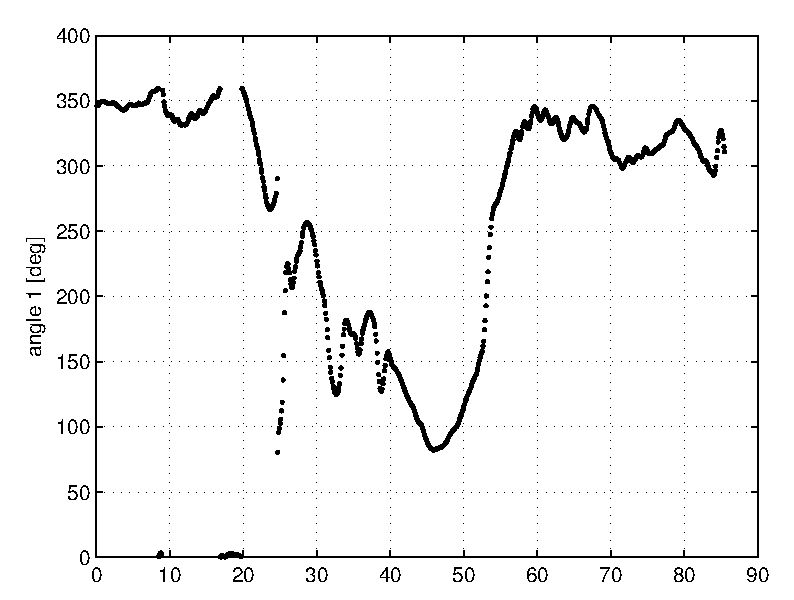
\includegraphics[width=0.45\textwidth]{methodology/fig/angle1.eps}}
    \subfigure[Second angular signal.]{\label{fig:second}
    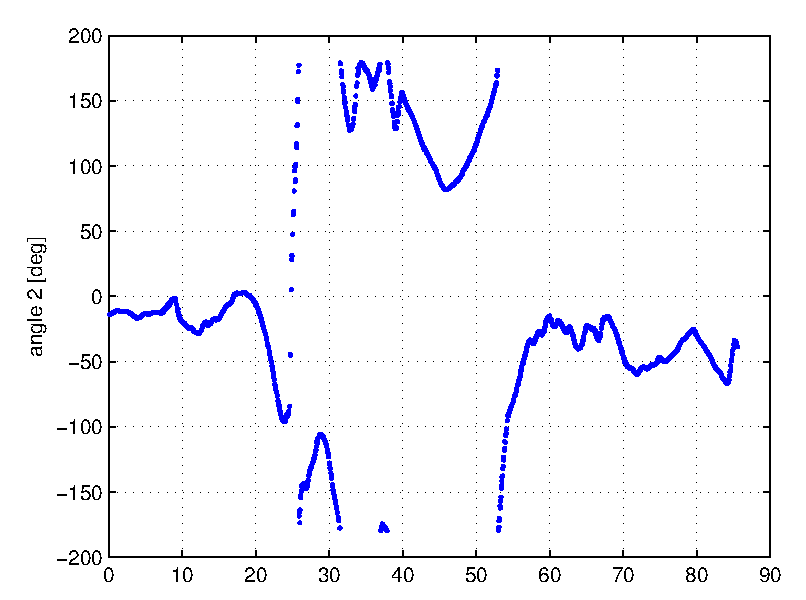
\includegraphics[width=0.45\textwidth]{methodology/fig/angle2.eps}}  \\
    \subfigure[Difference of two signals. ]   {\label{fig:diff}   
    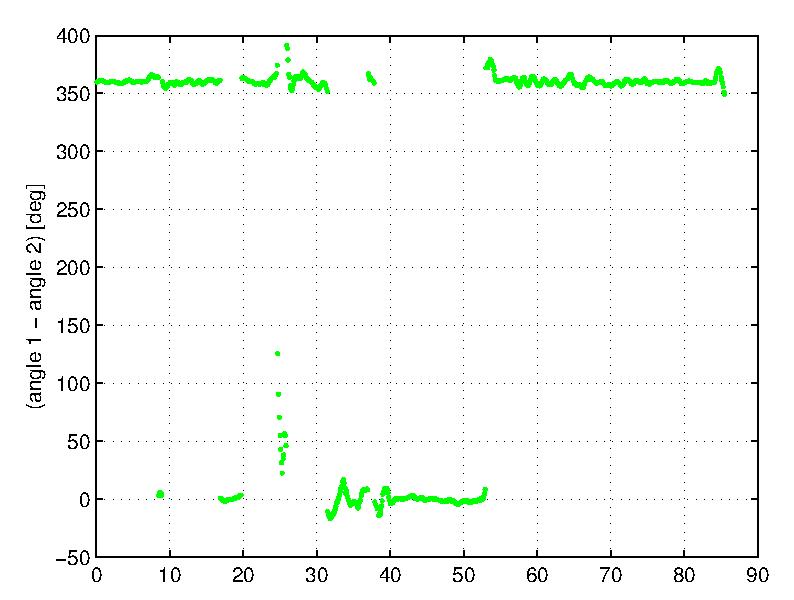
\includegraphics[width=0.45\textwidth]{methodology/fig/angle1-2.eps}}
    \subfigure[Angle wrapping in $0/+360$ and $-180/+180$. Angular values used as gain should be wrapped around zero.]{\label{fig:diff-wrap}
    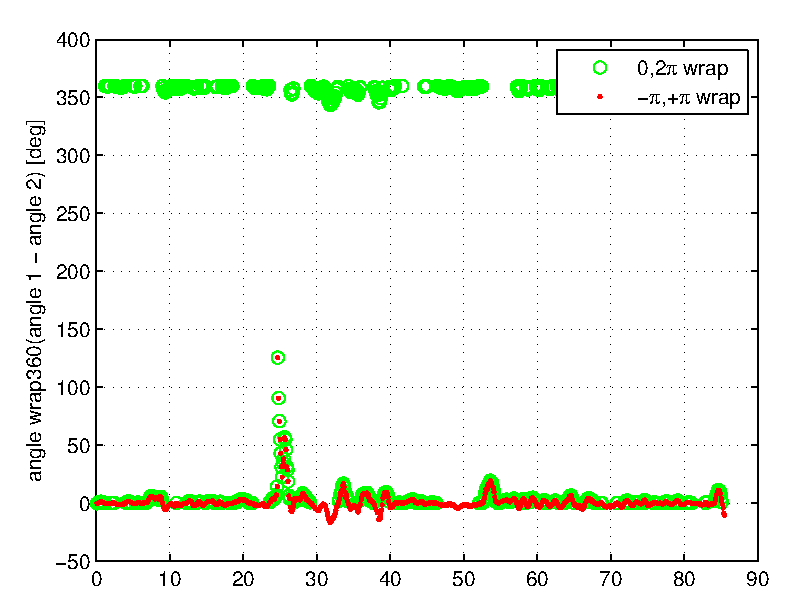
\includegraphics[width=0.45\textwidth]{methodology/fig/wrapangle1-2.eps}}   
  \end{center}
  \caption{Importance of angle wrapping.}
  \vspace{-10pt}
  \label{fig:ang-wrapping}
\end{figure} 